\clearpage
\newpage

\section{Problem 6 (20 pts)}

\subsection{Part 1:}
\begin{enumerate}
    \item In order to prove that the binary relation R: \textit{"is of type"} in the domain of types in the Java API is \textit{a partial order}, it is necessary to prove that binary relation R satisfies three properties: reflexivity, antisymmetry, and transitivity. Consider set A is the domain of types in the Java API.
    \begin{itemize}
        \item \textbf{Reflexivity: } When $\forall a \in$ A: aRa. In this case, for any type a in A, a is type of a. This is true since every type is inherently of its own type.
        \item \textbf{Antisymmetry: } When $\forall a, b \in A: (aRb \wedge bRa) \rightarrow a = b$. If a is of type b and b is of type a, then a must be equal to b. This property is satisfied as in Java, two types are of type to each other only if they are equal. 
        \item \textbf{Transitivity: } When $\forall a, b, c \in A: (aRb \wedge bRc) \rightarrow aRc$. If type a is type of b and type b is type of c, then type a is type of c. This property is true because if a class or interface or extends another type, and that type implements of extends another type (is type of another type), then the first type is also of the last type. \\ \\
        Therefore, the binary relation R is a partial order as it satisfies three properties: reflexivity, antisymmetry, and transitivity. 
    \end{itemize}
    \item To prove ($V_{1}$, R) is a poset, it is neccessary to procve that the binary relation R is a partial order over $V_{1}$. It means that the relation must satisfy three properties: reflexivity, antisymmetry, transitivity. 
    \begin{itemize}
        \item \textbf{Reflexivity: } When $\forall a \in$ $V_{1}$: aRa. In this case, for any type a in $V_{1}$, a is type of a. This is true since every type is of its own type. Which means that the provided edges have self-loops.
        \item \textbf{Antisymmetry: } When $\forall a, b \in V_{1}: (aRb \wedge bRa) \rightarrow a = b$. If a is of type b and b is of type a, then a must be equal to b. From the provided edges, it is observed that there are no two different vertices a, b such that aRb and bRa hold. E.g: There are no (HashMap, AbstractMap) and (AbstractMap, HashMap) hold. Therefore, antisymmetry is satisfied.
        \item \textbf{Transitivity: } When $\forall a, b, c \in V_{1}: (aRb \wedge bRc) \rightarrow aRc$. If type a is type of b and type b is type of c, then type a is type of c. According to the provided edges, there are no vertices a, b,c such that aRb and bRc. E.g: There are no sets of edges such that (LinkedHashMap, HashMap), (HashMap, AbstractMap), and (LinkedHashMap, AbstractMap). Therefore, the relation is transitive.\\ \\
        Therefore, ($V_{1}$, R) is a poset as it satisfies three properties: reflexivity, antisymmetry, and transitivity. 
    \end{itemize}
    \item Hasse Diagram \\
    \begin{figure}[hbt!]
        \centering
        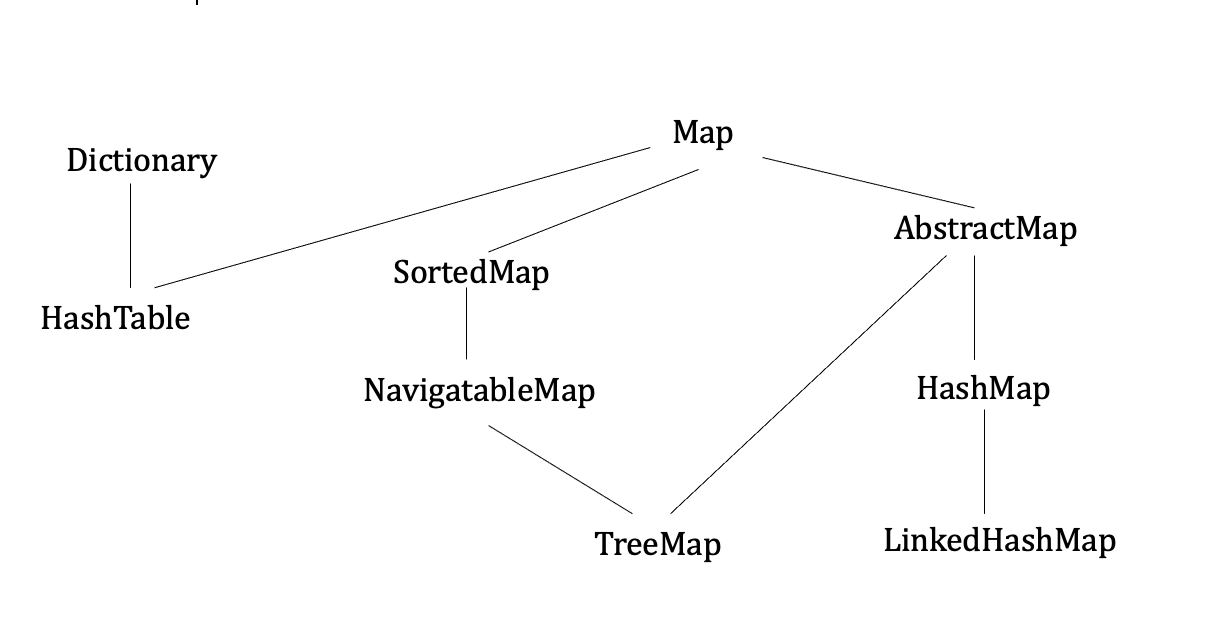
\includegraphics[scale=0.5]{HasseProblem613.png}
        \caption{Hasse Diagram for Problem 6.1.3}
        \label{fig:Hasse613}
    \end{figure}\\
    From Figure \ref{fig:Hasse613}, there is three minimal elements (HashTable, TreeMap, and LinkedHashMap), and two maximal elements (Dictionary, Map).
\end{enumerate}
\subsection{Part 2:}
\begin{enumerate}
    \item To prove that $\subseteq$ (is subset of) is a partial order, it is needed to indicate that $\subseteq$ satisfies three properties: reflexivity, antisymmetry, and transitivity. Consider A is the domain of sets.
    \begin{itemize}
        \item \textbf{Reflexivity: } When $\forall a \in$ A: a$\subseteq$a. This property is satisfied since every set is a subset of itself.    
        \item \textbf{Antisymmetry: } When $\forall a, b \in A: (a$\subseteq$b \wedge b$\subseteq$a) \rightarrow a = b$. This property is true because if two sets are subsets of each other, they must be equal.
        \item \textbf{Transitivity:} When $\forall a, b, c \in A: (a\subseteq b \wedge b\subseteq c) \rightarrow a\subseteq c$. This property holds its validity, because if a is a subset of b and b is a subset of c, a is a subset of c. \\ \\
        Therefore, $\subseteq$ is a partial order as it satisfies three properties: reflexivity, antisymmetry, transitivity.
    \end{itemize}
    \item \textit{P}($V_{2}$) is the power set of $V_{2}$ = \{a, b, c\}. This is the set containing all subsets of the set $V_{2}$. It is define as follows:\\ \\
    $\textit{P}\{a, b, c\} = \\
    \{ \\
    \emptyset, \\
    \{a\}, \{b\}, \{c\},\\
    \{a, b\}, \{a, c\}, \{b, c\},\\
    \{a, b, c\}\\
    \}\\ \\$
    To prove that ($\textit{P}(V_{2}), \subseteq$) is a poset, it is required to prove that the binary relation $\subseteq$ is a partial order over the power set \textit{P}. It means that the binary relation $\subseteq$ must satisfy three properties: reflexivity, antisymmetry, transitivity.
    \begin{itemize}
        \item \textbf{Reflexivity: } When $\forall a \in$ P: a$\subseteq$a. This property is satisfied because for every subset in P, it is a subset of itself. 
        \item \textbf{Antisymmetry: } When $\forall a, b \in P: (a$\subseteq$b \wedge  b$\subseteq$a) \rightarrow a = b$. This property is true because if two sets are subsets of each other, they must be equal. In this case, it is observed that there are not two subsets such as \{a, b\}, \{b, a\} in P. Therefore, this property is true.
        \item \textbf{Transitivity:} When $\forall a, b, c \in P: (a\subseteq b \wedge b\subseteq c) \rightarrow a\subseteq c$. This property is true, because if a is a subset of b and b is a subset of c, a is a subset of c. E.g: \{a\} is a subset of \{a, b\}, and \{a, b\} is a subset of \{a, b, c\}, then \{a\} is a subset of \{a, b, c\}. \{a\}, \{a, b\}, \{a, b, c\} are subsets of P. \\ \\
        Therefore, ($\textit{P}(V_{2}), \subseteq$) is a poset as it satisfies three properties: reflexivity, antisymmetry, transitivity. 
    \end{itemize}
    \item Hasse Diagram \\
    \begin{figure}[hbt!]
        \centering
        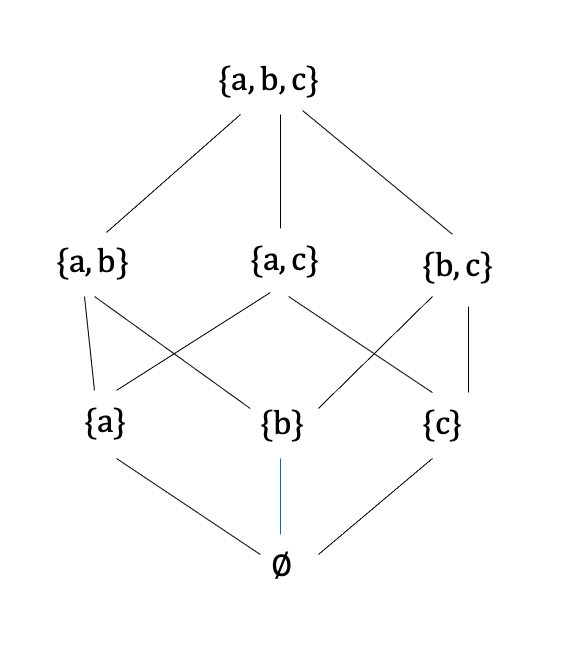
\includegraphics[scale=0.5]{HasseProblem63.png}
        \caption{Hasse Diagram for Problem 6.2.3}
        \label{fig:Hasse63}
    \end{figure}\\
    From Figure \ref{fig:Hasse63} There is one minimal element, $\emptyset$ and one maximal element, \{a, b, c\}.

\end{enumerate}
\subsection{Part 3: }
\textbf{Mapping: }Mapping map is a \textit{partial function} as it is a function defined for some subset of $V_{1}$. It does not force the mapping of every element of $V_{1}$ to an element of $\textit{P}(V_{2})$\\ \\
\textbf{Injectivity: }The function is not injective because it does not satisfy the condition of injectivity such that $\forall a, b (a \neq b \rightarrow f(a) \neq f(b))$. In this case, Dictionary and AbstractMap are mapped to the same element (\{a, b, c\}). \\ \\
\textbf{Surjectivity: }The fucntion is surjective as it is the case that $\forall b \exists a (f(a) = b)$. It can be observed that for each element of the codomain, it is mapped with at least one element in the domain. \\ \\
\textbf{Bijection: }By definition, the function is not bijective as it is not the case that both injectivity and surjectivity are satisfied. \\ \\ 
\textbf{Order preserving: }This function is not order-preserving as it is not the case that x $\prec$ y in domain of map, implies f(x) $\prec$ f(y)in in codomain of map. In this case, TreeMap is a predecessor of AbstractMap, but $\emptyset$ is not a predecessor of \{a, b, c\}\\ \\
\textbf{Order reflecting: }: This function is order reflecting because the predecessor relationship between elements in the codomain is reflected by their pre-images in the domain. \\ \\
\textbf{Order embedding: }By definition, the function is not order embedding as it is not the case that the function is both order preserving and order reflecting.\\ \\
\textbf{Isomorphism: }By definition, the function is not isomorphic as it is not the case that the function is order embedding and surjective.\\